\section{CONJUNTO DO PRODUTO (ENTREGA 3)}\label{sec:conjunto_produto}

% Os desenhos desta seção são gerados por imagens/conjunto_produto/gerar_conjunto.py.
% Para mudar uma medida, altere o dicionário P do script e rode de novo.
% TODO (equipe): o pino atravessa o tecido, como na alternativa escolhida na Entrega 2.
%   O modelo digital do protótipo também foi montado com o pino ao lado do tecido (prende só pelos dentes).
%   Se a equipe adotar essa variante, rever os itens "Retenção" das tabelas desta seção e a posição do pino no desenho.
% TODO (equipe): a massa do conjunto (E11) ainda não foi estimada.
% TODO (equipe): incluir a referência do campo dos destacadores comerciais (4.500 G) quando a fonte for escolhida.

Esta seção apresenta o conjunto do Tag\&Go: a posição de cada componente, as dimensões principais e as interfaces entre os sistemas. O ponto de partida é o desenho reformulado da Entrega 2 (Figura~\ref{fig:reform_desenho}), que era um esquema sem escala. Seguindo \citeonline{rozenfeld2006gestao}, a equipe deu corpo a cada bloco da arquitetura em dois passos: identificou os aspectos críticos de cada sistema e fixou seus parâmetros principais de forma, dimensão e capacidade. Depois conferiu se as geometrias cabem no envelope e como energia, sinal e força passam de um sistema ao outro.

O arranjo foi verificado em um modelo digital do protótipo, construído com as medidas dos componentes de mercado. Nenhuma medida desta seção vem de ensaio em bancada: cada valor está identificado como proveniente do modelo digital ou como estimativa.

\subsection{Revisão da concepção}
\label{subsec:conj_revisao}

A alternativa escolhida na Entrega 2 retinha a peça com pino e embreagem de esferas, bloqueava o carretel com um came e liberava com uma mola de torção armada, solta por um gatilho e por um microatuador. Ao detalhar essa alternativa, a equipe encontrou três parâmetros que não conseguiu dimensionar: a força da mola, o curso do came e o consumo do microatuador para retirar o gatilho sob carga. Por isso a liberação foi revista, e a revisão levou a outros ajustes. A Tabela~\ref{tab:conj_revisao} compara as duas concepções.

\begin{table}[htbp]
    \centering
    \caption{Concepção da Entrega 2 e concepção revisada}
    \label{tab:conj_revisao}
    \footnotesize
    \renewcommand{\arraystretch}{1.3}
    \begin{tabularx}{\textwidth}{@{}
        >{\RaggedRight\arraybackslash}p{2.3cm}
        >{\RaggedRight\arraybackslash}p{3.6cm}
        >{\RaggedRight\arraybackslash}p{4.0cm}
        >{\RaggedRight\arraybackslash}X@{}}
        \toprule
        \textbf{Função} & \textbf{Entrega 2} & \textbf{Concepção revisada} & \textbf{Motivo} \\
        \midrule
        Prender na peça & Haste solta, colocada pelo funcionário & Garra articulada com dentes e revestimento de elastômero, que leva o pino & O pino deixa de ser uma peça solta, e a abertura da garra mostra a liberação ao comprador \\
        Reter & Pino com embreagem de esferas & Mantida & Princípio consolidado nas etiquetas rígidas. Retém sem consumir energia \\
        Bloquear & Came de bloqueio com batente & Dispensado & A embreagem só se abre com o ímã sob ela. O ímã fica afastado até a autorização \\
        Liberar & Mola de torção com gatilho e microatuador & Microatuador rotativo que leva três ímãs até a posição sob a embreagem & Mesmo princípio dos destacadores de caixa. Elimina a mola armada, cujo dimensionamento ficou em aberto \\
        Identificar & Código 2D gravado & Mantida & O endereço do código é fixo. O servidor escolhe a página pelo estado do dispositivo \\
        Autorizar & Bobina receptora, pelo toque do celular & Placa de controle com rádio, que consulta o servidor & A ordem de liberação parte do servidor depois do pagamento. O celular não precisa encostar no dispositivo \\
        Indicar & Anel de LEDs & Três LEDs: vermelho, amarelo e verde & Um LED por estado: travado, em recarga e liberado \\
        Suprir energia & Célula recarregada por indução & Mantida, com chave que detecta a base de recarga & A chave informa a recarga à placa de controle \\
        \bottomrule
    \end{tabularx}
    \source{Elaborado pelos autores (2026).}
\end{table}

Duas alternativas foram avaliadas e descartadas no modelo digital. A primeira exibia o código 2D em uma tela, com um botão para o funcionário iniciar o cadastro. Ela acrescentava dois componentes, dez ligações e consumo, e o código gravado cumpre a mesma função quando o servidor guarda o estado do dispositivo. A segunda travava a garra com uma lingueta de plástico puxada pelo microatuador. Ela dispensa os ímãs, mas trava em uma única posição e troca um componente consolidado por uma peça própria sujeita a desgaste. Ela permanece como alternativa caso o campo dos ímãs não seja suficiente.

\subsection{Aspectos críticos e parâmetros principais}
\label{subsec:conj_criticos}

A Tabela~\ref{tab:conj_criticos} registra, para cada sistema, o aspecto que mais condiciona o projeto e os parâmetros que foram fixados. Os códigos dos sistemas são os da estrutura do produto (Seção~\ref{sec:estrutura_produto}).

\begin{table}[htbp]
    \centering
    \caption{Aspectos críticos e parâmetros principais de cada sistema}
    \label{tab:conj_criticos}
    \footnotesize
    \renewcommand{\arraystretch}{1.3}
    \begin{tabularx}{\textwidth}{@{}
        >{\RaggedRight\arraybackslash}p{2.6cm}
        >{\RaggedRight\arraybackslash}X
        >{\RaggedRight\arraybackslash}X@{}}
        \toprule
        \textbf{Sistema} & \textbf{Aspecto crítico} & \textbf{Parâmetros principais} \\
        \midrule
        Estrutura e fechamento (TG-100) & Montagem: a distância entre a embreagem e o eixo do microatuador não pode depender do fechamento da tampa & Suporte único para a embreagem e o microatuador. Parede de 2,0 mm e fundo de 1,5 mm sobre a bobina (estimativas) \\
        Retenção (TG-200) & Funcionamento: a força para arrancar a peça (E12) depende da embreagem e do atrito dos dentes com o tecido & Embreagem de $\varnothing$~13~$\times$~11 mm e pino de $\varnothing$~1,2~$\times$~16 mm (modelo digital). Garra de 52~$\times$~32~$\times$~6 mm, com abertura de cerca de 30$^\circ$ \\
        Liberação (TG-300) & Funcionamento: o campo sob a embreagem precisa recolher o carretel através da prateleira, e o microatuador precisa deslocar os ímãs, que são atraídos pela embreagem & Três ímãs de $\varnothing$~10~$\times$~4 mm, a 0,2 mm de uma prateleira de 0,8 mm. Braço de 16 mm e curso de 90$^\circ$ (modelo digital). Torque do microatuador a definir \\
        Indicação (TG-400) & Custo e montagem: os LEDs atravessam a tampa e pedem vedação & Três LEDs de $\varnothing$~3 mm, afastados 12 mm entre si (estimativa) \\
        Controle e energia (TG-500) & Funcionamento: os ímãs e a embreagem, perto da bobina, prejudicam a recarga. Descarte: a célula precisa sair sem destruir a carcaça & Afastamento mínimo de 30 mm entre ímã e bobina (estimativa). Célula de 50~$\times$~34~$\times$~6 mm e bobina de $\varnothing$~40 mm (estimativas de catálogo). Tampa presa por quatro parafusos \\
        \bottomrule
    \end{tabularx}
    \source{Elaborado pelos autores (2026).}
\end{table}

O parâmetro de maior risco é o campo magnético. Os destacadores de loja para etiquetas comuns são vendidos com campo de cerca de 4.500~G. Pelo cálculo da equipe, a pilha de três ímãs alcança cerca de 6.500~G na face e cerca de 5.200~G a 1 mm, que é a distância somada da folga e da prateleira. A margem é pequena, e o valor é uma estimativa de cálculo, ainda não verificada em ensaio. O torque do microatuador depende da força com que a embreagem atrai os ímãs e também só será fixado depois do ensaio.

\subsection{Desenho de conjunto}
\label{subsec:conj_desenho}

A Figura~\ref{fig:conj_desenho} mostra o conjunto em duas vistas na mesma escala, alinhadas pelo comprimento: a vista superior, com a tampa tratada como transparente, e o corte A--A, que passa pelo eixo do pino. Os números dos balões correspondem aos códigos da estrutura do produto (Tabela~\ref{tab:estrut_lista}).

\begin{figure}[p]
    \centering
    \caption{Desenho de conjunto do Tag\&Go, em vista superior e em corte pelo eixo do pino. Cotas em mm}
    \label{fig:conj_desenho}
    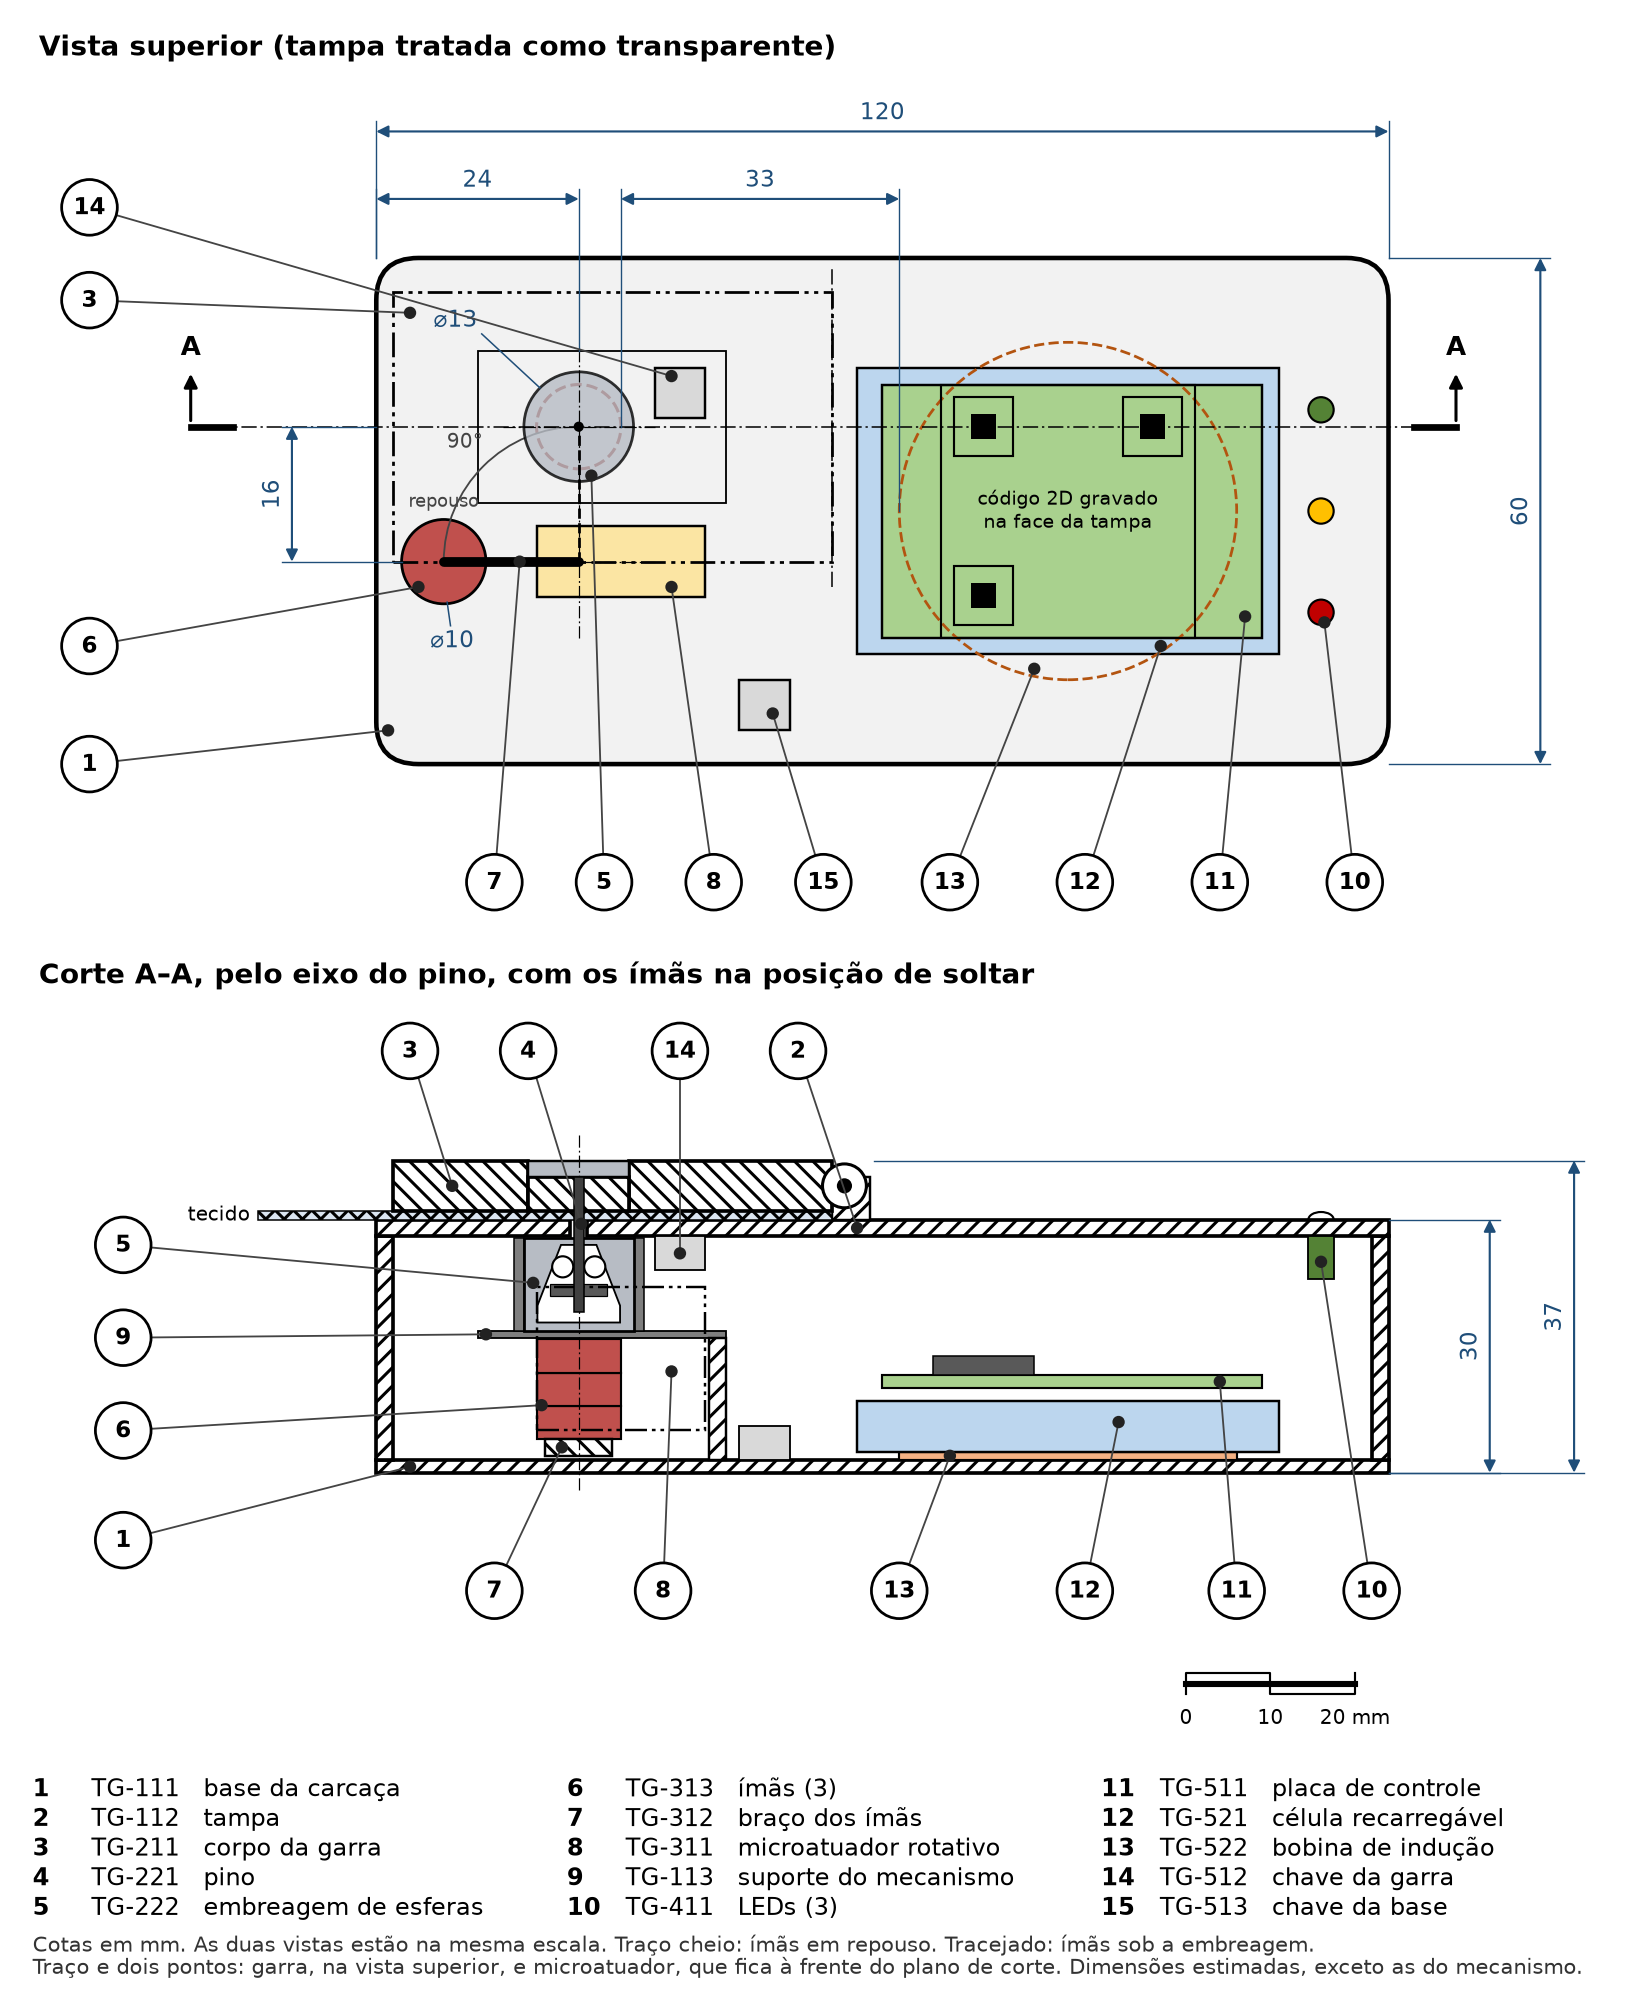
\includegraphics[width=\textwidth]{imagens/conjunto_produto/conjunto_produto.png}
    \source{Elaborado pelos autores (2026). Figura gerada com apoio de ferramenta de IA.}
\end{figure}

O dispositivo tem duas zonas. A zona do mecanismo ocupa os primeiros 41 mm do comprimento e reúne a embreagem, o braço com os ímãs e o microatuador, montados no suporte do mecanismo. A zona da eletrônica ocupa o restante e empilha, de baixo para cima, a bobina de indução, a célula e a placa de controle. Os LEDs ficam na extremidade oposta ao mecanismo, e o código 2D é gravado na face da tampa, sobre a zona da eletrônica. A garra fica sobre a tampa, do lado do mecanismo.

A separação em zonas decorre do afastamento entre os ímãs e a bobina. No arranjo adotado, a borda do ímã na posição de soltar fica a 33 mm da borda da bobina, cota indicada na vista superior. Em repouso, os ímãs ficam ainda mais afastados da bobina e a 16 mm do eixo da embreagem, fora do alcance do carretel.

No corte, a garra está fechada sobre o tecido. O pino, fixado na garra, atravessa o tecido e o furo da tampa e entra na embreagem. Os ímãs aparecem sob a embreagem, na posição de soltar. O microatuador fica à frente do plano de corte e está desenhado em linha fantasma.

A Figura~\ref{fig:conj_camadas} separa o conjunto em camadas, na ordem em que as peças entram na base. A mesma sequência servirá de ponto de partida para o plano de montagem.

\begin{figure}[htbp]
    \centering
    \caption{Vista em camadas do conjunto, na ordem de montagem}
    \label{fig:conj_camadas}
    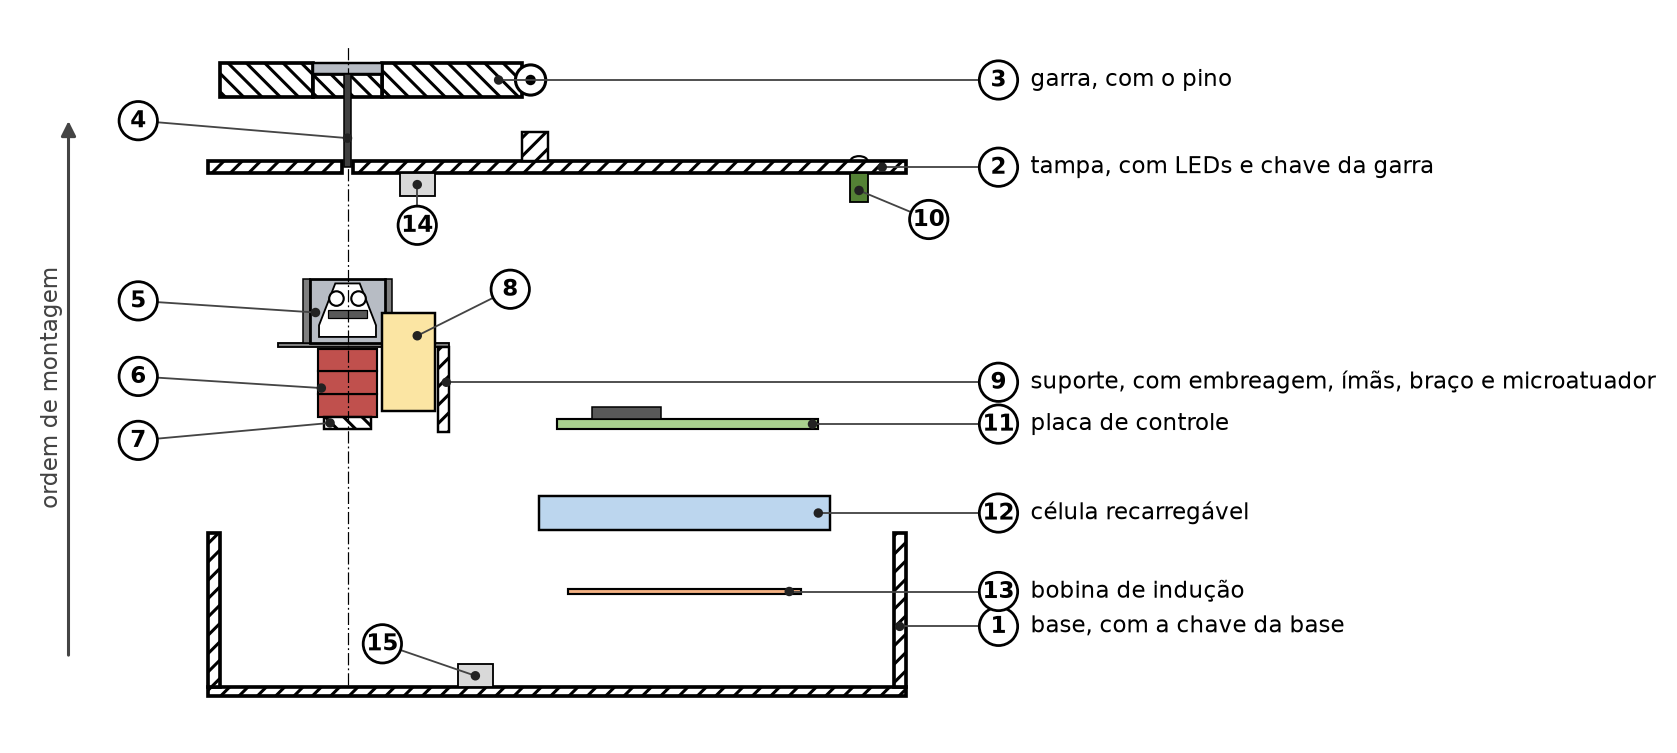
\includegraphics[width=\textwidth]{imagens/conjunto_produto/conjunto_camadas.png}
    \source{Elaborado pelos autores (2026). Figura gerada com apoio de ferramenta de IA.}
\end{figure}

A Figura~\ref{fig:conj_modelo} mostra o modelo digital do protótipo. Ele é maior que o produto, porque usa componentes de mercado sem solda: a caixa mede 210~$\times$~76~$\times$~54 mm, contra 120~$\times$~60~$\times$~30 mm do conjunto desta seção. O mecanismo, porém, é o mesmo e tem as mesmas medidas. O modelo foi usado para conferir o percurso dos ímãs, as folgas e a ordem de montagem.

\begin{figure}[htbp]
    \centering
    \caption{Modelo digital do protótipo, com a garra aberta. A carcaça está transparente para mostrar o mecanismo}
    \label{fig:conj_modelo}
    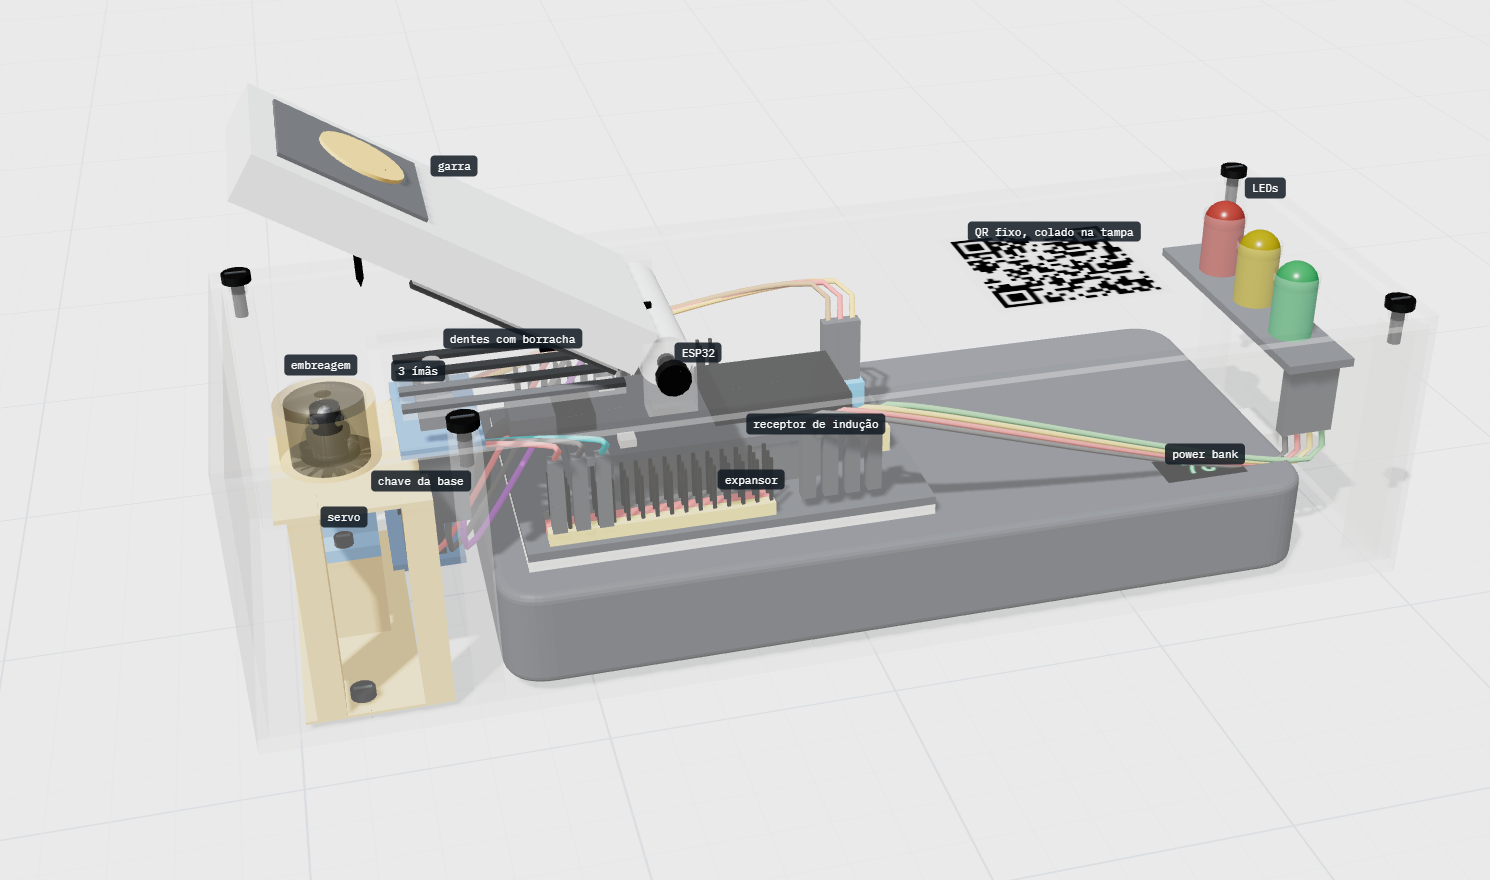
\includegraphics[width=0.92\textwidth]{imagens/conjunto_produto/modelo_digital_prototipo.png}
    \source{Elaborado pelos autores (2026). Modelo gerado com apoio de ferramenta de IA.}
\end{figure}

\subsection{Interfaces entre os sistemas}
\label{subsec:conj_interfaces}

A Tabela~\ref{tab:conj_interfaces} lista o que passa de um sistema a outro. A interface entre a liberação e a retenção é a única sem contato: o campo dos ímãs atravessa a prateleira do suporte e age sobre o carretel da embreagem.

\begin{table}[htbp]
    \centering
    \caption{Interfaces entre os sistemas do Tag\&Go}
    \label{tab:conj_interfaces}
    \footnotesize
    \renewcommand{\arraystretch}{1.3}
    \begin{tabularx}{\textwidth}{@{}
        >{\RaggedRight\arraybackslash}p{3.0cm}
        >{\RaggedRight\arraybackslash}p{3.0cm}
        >{\RaggedRight\arraybackslash}p{1.5cm}
        >{\RaggedRight\arraybackslash}X@{}}
        \toprule
        \textbf{De} & \textbf{Para} & \textbf{Fluxo} & \textbf{Descrição} \\
        \midrule
        Ímãs (TG-313) & Embreagem (TG-222) & Força & O campo recolhe o carretel através da prateleira de 0,8 mm, e as esferas liberam o pino \\
        Mola de abertura (TG-213) & Corpo da garra (TG-211) & Força & Com o pino livre, a mola abre a garra em cerca de 30$^\circ$ \\
        Corpo da garra (TG-211) & Chave da garra (TG-512) & Força & A garra fechada pressiona a chave, através de um furo na tampa \\
        Chave da garra (TG-512) & Placa de controle (TG-511) & Sinal & Informa se a garra está fechada \\
        Chave da base (TG-513) & Placa de controle (TG-511) & Sinal & Informa se o dispositivo está na base de recarga \\
        Placa de controle (TG-511) & Microatuador (TG-311) & Sinal e energia & Comanda o giro de 90$^\circ$ e o retorno \\
        Placa de controle (TG-511) & LEDs (TG-411) & Sinal & Acende o LED do estado atual \\
        Bobina (TG-522) & Célula (TG-521) & Energia & Recarrega a célula, através do fundo de 1,5 mm \\
        Célula (TG-521) & Placa de controle (TG-511) & Energia & Alimenta a placa, que distribui a energia \\
        Servidor (externo) & Placa de controle (TG-511) & Sinal & Recebe o estado das chaves e envia a ordem de liberação, por rádio \\
        Código 2D (na TG-112) & Celular (externo) & Sinal & O celular lê o endereço do dispositivo e abre a página de cadastro ou de compra \\
        \bottomrule
    \end{tabularx}
    \source{Elaborado pelos autores (2026).}
\end{table}

\subsection{Dimensões principais}
\label{subsec:conj_dimensoes}

A Tabela~\ref{tab:conj_dimensoes} reúne as dimensões do conjunto e dos componentes que determinam o envelope. As medidas marcadas como modelo digital são as dos componentes de mercado usados no modelo do protótipo. As demais são estimativas de catálogo ou resultam do arranjo.

\begin{table}[htbp]
    \centering
    \caption{Dimensões principais do conjunto}
    \label{tab:conj_dimensoes}
    \footnotesize
    \renewcommand{\arraystretch}{1.3}
    \begin{tabularx}{\textwidth}{@{}
        >{\RaggedRight\arraybackslash}p{6.2cm}
        >{\RaggedRight\arraybackslash}p{3.6cm}
        >{\RaggedRight\arraybackslash}X@{}}
        \toprule
        \textbf{Item} & \textbf{Dimensão (mm)} & \textbf{Origem do valor} \\
        \midrule
        Carcaça fechada (comprimento, largura e altura) & 120 $\times$ 60 $\times$ 30 & Estimativa, resultado do arranjo \\
        Altura com a garra fechada & 37 & Estimativa, resultado do arranjo \\
        Parede, fundo e tampa & 2,0; 1,5 e 2,0 & Estimativa \\
        Embreagem de esferas & $\varnothing$ 13 $\times$ 11 & Modelo digital \\
        Pino & $\varnothing$ 1,2 $\times$ 16 & Modelo digital \\
        Ímã (cada um dos três) & $\varnothing$ 10 $\times$ 4 & Modelo digital \\
        Prateleira do suporte, sob a embreagem & 0,8 de espessura & Modelo digital \\
        Folga entre os ímãs e a prateleira & 0,2 & Modelo digital \\
        Distância entre o eixo do microatuador e o do pino & 16 & Modelo digital \\
        Curso do braço & 90$^\circ$ & Modelo digital \\
        Posição do eixo do pino, a partir da extremidade & 24 & Estimativa \\
        Afastamento entre o ímã, na posição de soltar, e a bobina & 33 & Estimativa, resultado do arranjo \\
        Microatuador rotativo & 20 $\times$ 8,5 $\times$ 17 & Estimativa de catálogo \\
        Corpo da garra & 52 $\times$ 32 $\times$ 6 & Estimativa \\
        Célula recarregável & 50 $\times$ 34 $\times$ 6 & Estimativa de catálogo \\
        Bobina de indução & $\varnothing$ 40 $\times$ 1 & Estimativa de catálogo \\
        Placa de controle & 45 $\times$ 30 $\times$ 1,6 & Estimativa \\
        Área do código 2D gravado & 30 $\times$ 30 & Estimativa \\
        \bottomrule
    \end{tabularx}
    \source{Elaborado pelos autores (2026).}
\end{table}

\subsection{Confronto com a especificação de dimensões}
\label{subsec:conj_confronto}

A especificação E10 fixou o envelope do dispositivo em 98~$\times$~82~$\times$~26 mm. O conjunto atende à largura, com 60 mm, e não atende ao comprimento nem à altura: excede o comprimento em 22 mm e a altura em 4 mm, ou em 11 mm com a garra. O volume da carcaça é de cerca de 216~cm$^3$, contra 209~cm$^3$ do envelope especificado.

A altura é determinada pela pilha do mecanismo: a embreagem (11 mm), a prateleira (0,8 mm), os três ímãs (12 mm) e o braço (2 mm) somam cerca de 26 mm, aos quais se acrescentam o fundo e a tampa. O comprimento é determinado pelo afastamento entre os ímãs e a bobina e pelo comprimento da célula. A equipe identificou três caminhos de redução, a avaliar no projeto detalhado:

\begin{itemize}
    \item substituir os três ímãs empilhados por um ímã único de maior grau, o que reduz a altura da pilha;
    \item medir o afastamento mínimo real entre o ímã e a bobina, hoje estimado em 30 mm, o que pode encurtar o comprimento;
    \item escolher uma célula mais curta, já que a retirada da tela reduziu o consumo previsto.
\end{itemize}

Até que esses caminhos sejam avaliados, a especificação E10 fica registrada como não atendida em comprimento e em altura.
